
\subsection{Proceso de atención al paciente y actualización de información}

La gestión clínico-administrativa por paciente en el Centro Odontológico Bellidental se realiza mediante un esquema tradicional basado en soportes de papel, hojas de cálculo independientes y canales informales de comunicación. Este flujo de trabajo se subdivide en dos componentes principales, de los cuales se excluye de forma explícita el tiempo clínico de la consulta: la Etapa 1: Gestión en la atención, que corresponde a lo que ocurre con el paciente presente (diagrama 1, $T_{E1} = 6{,}3$ min), y la Etapa 2: Gestión documental diferida, referente al tratamiento posterior de los datos de esa misma atención (diagrama 2, $T_{E2} = 7{,}32$ min).

\subsubsection{Análisis del proceso actual}

En la operatividad diaria de la clínica, la atención del paciente y el manejo de su historial clínico se desarrollan en las siguientes etapas:

\begin{enumerate}[leftmargin=*]
    \item \textbf{Recepción e inicio de atención:} Al ingresar el paciente, la secretaria verifica su registro. Si es un usuario nuevo, se abre una ficha física preliminar de papel para anotar los datos de filiación y antecedentes médicos básicos. Si es un paciente recurrente, se busca su carpeta en el archivo de recepción.
    
    \item \textbf{Verificación de agendamiento:} La secretaria confirma la cita en la aplicación Google Calendar, donde los turnos están organizados por colores según el profesional asignado. Al mismo tiempo, atiende las solicitudes de confirmación y cambio de citas que ingresan por WhatsApp al teléfono corporativo.
    
    \item \textbf{Atención clínica y anamnesis:} El paciente ingresa al consultorio y el odontólogo recibe la ficha física. Debido a que la información inicial suele ser concisa, el profesional reinterroga al paciente sobre sus antecedentes de salud. Posterior a la revisión clínica, dibuja a mano el odontograma en el Formulario 033 oficial del Ministerio de Salud Pública, aplicando la convención de color rojo para tratamientos pendientes y azul para los ejecutados.
    
    \item \textbf{Procedimiento y prescripción médica:} Finalizada la intervención, si el paciente requiere medicación, el odontólogo escribe la receta a mano, indicando el fármaco, la dosis y el código diagnóstico de la Clasificación Internacional de Enfermedades. Al terminar, comunica verbalmente a la secretaria los procedimientos efectuados y le entrega la ficha con las notas manuscritas.
    
    \item \textbf{Cierre de atención y agendamiento:} En recepción, la secretaria realiza el cobro, registra en una hoja auxiliar los valores pagados y saldos pendientes, acuerda la fecha del próximo turno y lo asigna en Google Calendar.
    
    \item \textbf{Actualización diferida de fichas:} La secretaria no digita la información en tiempo real durante la consulta. En el bloque vespertino o al cierre del día, dedica entre 120 y 180 minutos a recopilar las fichas diarias. En esta etapa transcribe manualmente las notas y el odontograma al Formulario 033 físico definitivo y registra los datos administrativos en una hoja de cálculo en Microsoft Excel.
\end{enumerate}

Cabe destacar que en los diagramas BPMN que modelan estos procesos (Figuras~\ref{fig:bpmn1} y \ref{fig:bpmn2}) se representan únicamente las actividades que concentran tiempo, retrabajo o riesgo de error. Se han omitido los pasos de menor incidencia, como el llenado del encabezado institucional, la firma de la receta y de la tabla de control, o la coordinación de casos especiales por parte del odontólogo especialista.

\begin{figure}[H]
    \centering
    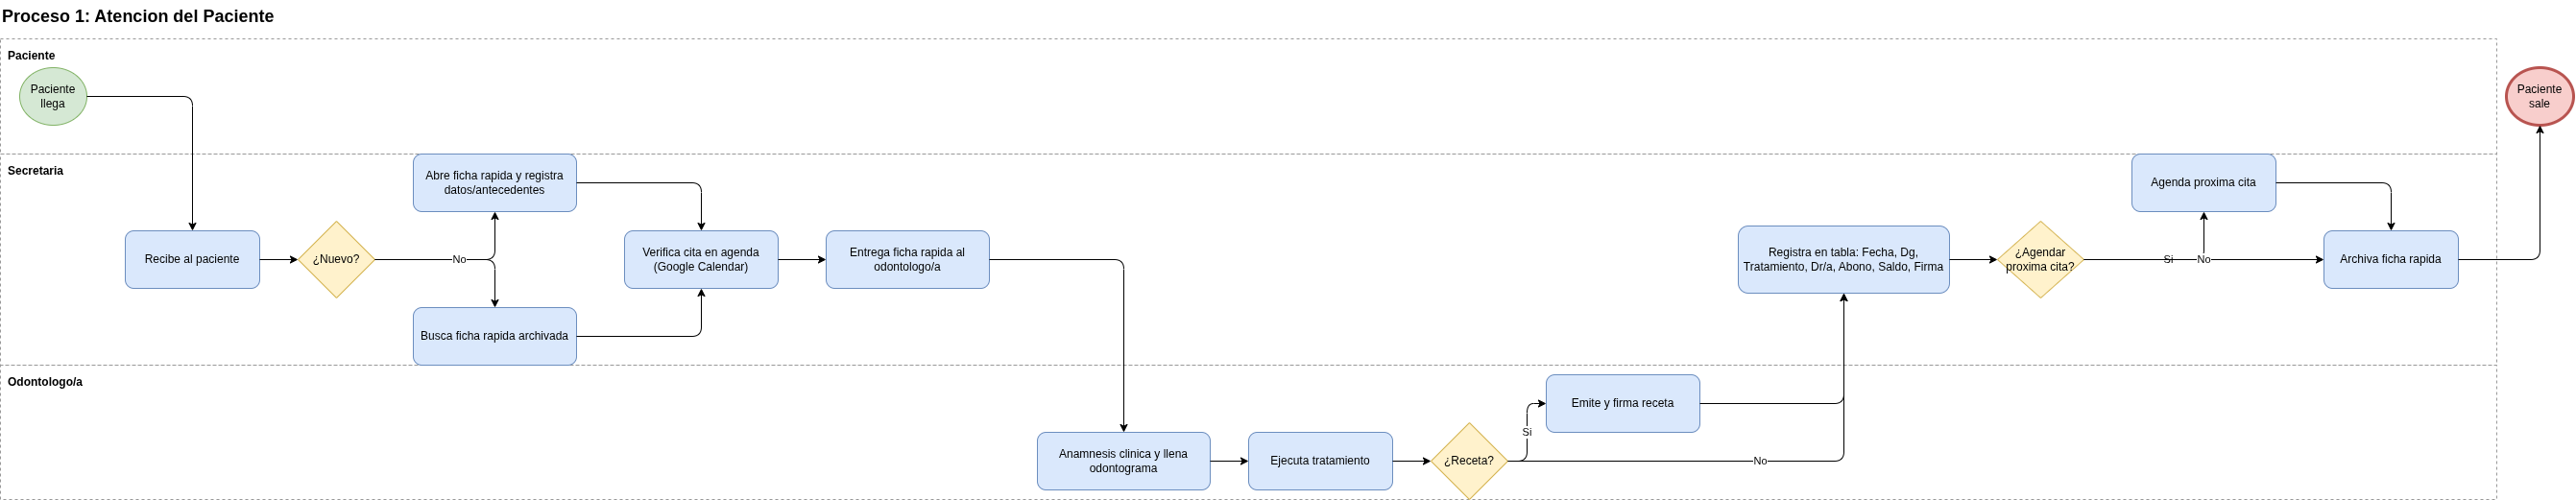
\includegraphics[width=\linewidth]{img/bpmn1.png}
    \caption{Etapa 1: Gestión en la atención.}
    \label{fig:bpmn1}
\end{figure}

\begin{figure}[H]
    \centering
    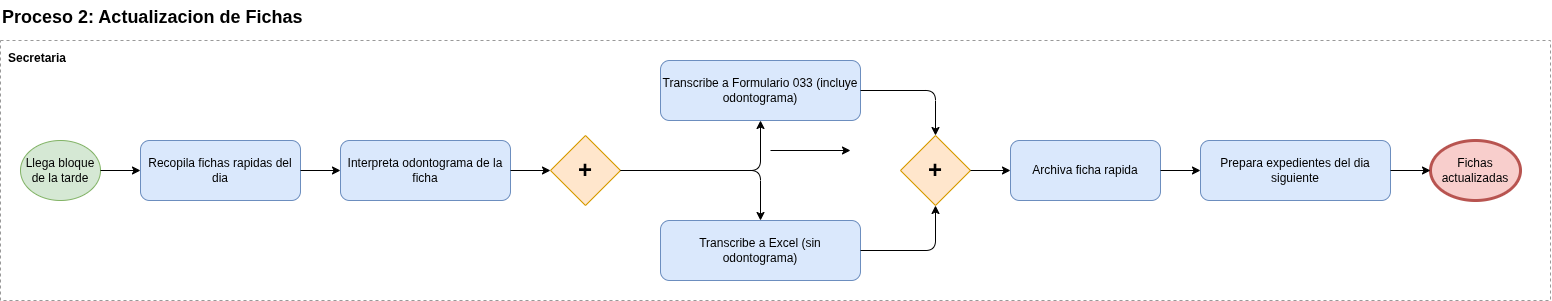
\includegraphics[width=\linewidth]{img/bpmn2.png}
    \caption{Etapa 2: Gestión documental diferida.}
    \label{fig:bpmn2}
\end{figure}

El diagnóstico del flujo de trabajo evidencia aspectos críticos en la operatividad, el registro de información y el cumplimiento normativo. A partir de los instrumentos de recolección de datos, se identifican las siguientes problemáticas en la gestión clínico-administrativa:

\begin{itemize}
    \item \textbf{Etapa 1: Gestión en la atención:} La acumulación de mensajes diarios en WhatsApp al inicio de la jornada genera demoras en la recepción. En el ámbito clínico, la confección manual de recetas y la búsqueda física de códigos diagnósticos restan tiempo a la atención. Según los datos de la ficha de observación, este tramo administrativo directo consume en promedio 6{,}3 minutos por paciente.
    
    \item \textbf{Etapa 2: Gestión documental diferida:} Representa el principal cuello de botella administrativo. La secretaria requiere retranscribir las fichas físicas al Formulario 033 y a una hoja de cálculo. La observación directa determinó que esta gestión documental diferida consume 7{,}32 minutos por ficha, sumando aproximadamente 190 minutos por jornada, lo que desvincula la atención presencial de la actualización del sistema informático y retrasa la disponibilidad de las historias clínicas.
\end{itemize}

Considerando ambas etapas ($T_{E1}$ y $T_{E2}$), el tiempo total destinado a la gestión administrativa por paciente asciende a 13{,}62 minutos, lo que evidencia la necesidad de optimización. Además, la falta de un sistema unificado origina las siguientes inconsistencias, errores y reprocesos:

\begin{itemize}
    \item \textbf{Cruces de agenda:} Ocurren duplicidades de turnos cuando los odontólogos confirman o modifican citas directamente con los pacientes por llamadas o mensajes personales, sin que la secretaria lo registre oportunamente en la agenda central.
    
    \item \textbf{Errores de transcripción:} El traspaso de datos desde las fichas preliminares al Formulario 033 definitivo y al archivo de Excel expone el historial clínico a errores de interpretación de la caligrafía o de la simbología del odontograma.
    
    \item \textbf{Falta de privacidad:} La recolección de antecedentes de salud en la sala de espera inhibe a algunos pacientes de declarar enfermedades o alergias. Esto obliga al odontólogo a repetir el cuestionario en el consultorio, prolongando la consulta.
\end{itemize}

\subsubsection{Análisis normativo}

El manejo actual de la información presenta vulnerabilidades frente a la legislación ecuatoriana. El sistema de información de la clínica está condicionado por tres referentes legales y normativos, frente a los cuales se identifican brechas de cumplimiento:

\begin{itemize}[leftmargin=*]
    \item \textbf{Formulario 033 y Acuerdo Ministerial 5216-A:} Esta normativa exige el registro secuencial, completo y legible del diagnóstico, tratamiento, evolución y prescripciones, incluyendo el odontograma y los códigos CIE-10, simultáneo a la atención del paciente. En la práctica actual, el odontograma se dibuja a mano y se retranscribe de manera diferida, y los códigos CIE-10 se buscan en una matriz física. Esto genera duplicidad de registros, riesgo de errores por mala interpretación de la caligrafía y disponibilidad limitada del historial para consultas inmediatas.
    
    \item \textbf{Reglamentos de la Historia Clínica Electrónica (Acuerdos 0009-2017 y 00115-2021):} Aplican a los establecimientos que emplean sistemas informáticos para la historia clínica y exigen principios de seguridad, integridad, exactitud, confidencialidad, no repudio y disponibilidad, requiriendo credenciales únicas por usuario. Actualmente, la clínica emplea expedientes de papel con firma manuscrita y una hoja de Excel como copia digital carente de controles de acceso individualizados. Esto impide garantizar la inalterabilidad de los datos, evidenciando la necesidad de implementar autenticación por roles, trazabilidad de registros (auditoría) y respaldos automáticos seguros.
    
    \item \textbf{Ley Orgánica de Protección de Datos Personales (LOPDP):} La legislación establece que los datos de salud conforman una categoría especial que requiere medidas rigurosas de seguridad, exactitud y confidencialidad. En la clínica, la falta de privacidad en recepción al recolectar antecedentes, el almacenamiento físico de fichas y el uso de mensajería comercial sin controles cifrados exponen la información a vulnerabilidades. Además, el Artículo 31 de la LOPDP demanda el consentimiento expreso del titular para tratar sus datos de salud. Dado que la clínica coordina citas por WhatsApp, se incurre en una brecha legal, pues no se cuenta con un aviso de privacidad ni consentimiento formal.
\end{itemize}

Estas brechas se traducen en requerimientos de cumplimiento obligatorio para el sistema propuesto: integración de un odontograma digital y un catálogo CIE-10, aseguramiento del registro simultáneo, autenticación por usuario con auditoría, y la inclusión de un aviso de privacidad de aceptación explícita para el uso del agente conversacional.

\subsubsection{Requerimientos del sistema}

Los requerimientos se levantaron a partir del análisis del proceso actual, las entrevistas al personal y las normativas aplicables. Se clasifican en funcionales, que describen lo que el sistema debe hacer, y no funcionales, que describen las condiciones de calidad bajo las que debe operar.

La Tabla~\ref{tab:requerimientos} detalla estos requerimientos. Se asignó prioridad alta a aquellos indispensables para resolver los problemas clínicos o exigidos por ley, y prioridad media a los que mejoran la operatividad.

\begingroup
\fontsize{9}{11}\selectfont
\renewcommand{\arraystretch}{1.2}
\setlength{\LTpre}{0pt}\setlength{\LTpost}{6pt}
\begin{longtable}{|c|p{9.5cm}|c|}
\caption{Requerimientos funcionales y no funcionales del sistema}
\label{tab:requerimientos} \\
\hline
\textbf{ID} & \textbf{Requerimiento} & \textbf{Prioridad} \\ \hline
\endfirsthead
\hline
\textbf{ID} & \textbf{Requerimiento} & \textbf{Prioridad} \\ \hline
\endhead
\hline
\endfoot

\multicolumn{3}{|l|}{\cellcolor{gray!10}\textbf{Requerimientos funcionales}} \\ \hline

RF01 & Historia clínica digital que replique el Formulario 033 del MSP campo por campo, sin variaciones, y que pueda imprimirse con todos los campos definidos. & Alta \\ \hline

RF02 & Odontograma digital interactivo: al seleccionar la pieza (11 a 48) y la cara se despliegan las opciones diagnósticas, usando rojo para lo pendiente y azul para lo ejecutado. & Alta \\ \hline

RF03 & Catálogo CIE-10 con buscador predictivo por texto o por prefijo (K0, K1), para evitar redigitación manual. & Alta \\ \hline

RF04 & Catálogo precargado de tratamientos y de fármacos con posología predefinida. & Alta \\ \hline

RF05 & Receta electrónica con autocompletado de fármaco y posología, asociada al código CIE-10 e impresa con espacio para firma. & Alta \\ \hline

RF06 & Consulta inmediata del historial, antecedentes y estado de tratamientos de cualquier paciente, con registro de antecedentes directamente en el consultorio. & Alta \\ \hline

RF07 & Agenda centralizada que conserve la lógica de colores de Google Calendar e impida cruces de citas. & Alta \\ \hline

RF08 & Registro de cobros con abono y saldo por sesión, y emisión de comprobante. & Media \\ \hline

RF09 & Agente conversacional en WhatsApp que agenda, reprograma y cancela citas consultando la agenda centralizada, y que admite que un familiar gestione la cita. & Alta \\ \hline

RF10 & Recordatorios automáticos previos a la cita, con solicitud de confirmación o reprogramación. & Alta \\ \hline

RF11 & Respuesta automática sobre horarios de atención, precios y formas de pago, derivando a la secretaria en casos complejos. & Media \\ \hline

RF12 & Aviso de privacidad y aceptación explícita del paciente antes de tratar sus datos por medio del agente en su primera interacción. & Alta \\ \hline

\multicolumn{3}{|l|}{\cellcolor{gray!10}\textbf{Requerimientos no funcionales}} \\ \hline

RNF01 & Persistencia de los datos: respaldos automáticos periódicos, exportación en formato abierto y ausencia de eliminación física de registros clínicos. & Alta \\ \hline

RNF02 & Seguridad y confidencialidad: credenciales únicas, roles de acceso (secretaria, odontólogo), comunicación cifrada y ausencia de datos clínicos sensibles en las respuestas del agente. & Alta \\ \hline

RNF03 & Auditoría: bitácora con usuario, fecha y hora de creación y modificación de cada registro o cita. & Alta \\ \hline

RNF04 & Disponibilidad y contingencia: acceso durante el horario de atención y agente disponible fuera de él. Ante una falla, la atención continúa con registro manual. & Media \\ \hline

RNF05 & Usabilidad: interfaz sencilla y eficiente que permita registrar durante la consulta sin desatender al paciente. & Alta \\ \hline

\end{longtable}
\endgroup

\subsubsection{Análisis para el agente conversacional}

El diseño e implementación del agente conversacional en WhatsApp responde a las necesidades de comunicación específicas detectadas en la encuesta a pacientes y a la saturación de mensajería reportada por recepción. La Tabla~\ref{tab:necesidades_comunicacion} resume los aspectos evaluados y la función requerida para el agente.

\begin{table}[H]
\centering
\caption{Necesidades de comunicación del paciente y funciones del agente}
\label{tab:necesidades_comunicacion}
\fontsize{9}{11}\selectfont
\renewcommand{\arraystretch}{1.2}
\begin{tabularx}{\linewidth}{|p{3.5cm}|p{3.8cm}|X|}
\hline
\textbf{Aspecto evaluado} & \textbf{Resultado (Pacientes)} & \textbf{Función del agente} \\ \hline
Facilidad para agendar & 50{,}5\,\% indicó que no fue fácil & Mostrar disponibilidad de horarios y permitir agendar de forma autónoma. \\ \hline
Respuesta lenta por WhatsApp & 60{,}0\,\% lo considera tardío & Responder de inmediato consultas frecuentes, a cualquier hora. \\ \hline
Olvido de la cita & 46{,}6\,\% ha olvidado su cita & Enviar recordatorios con fecha, hora y profesional. \\ \hline
Utilidad del recordatorio & 53{,}3\,\% lo considera muy útil & Pedir confirmación o reprogramación mediante el recordatorio. \\ \hline
Uso del asistente & 58{,}1\,\% está dispuesto a usarlo & Integrar flujos de agendamiento, reprogramación y cancelación. \\ \hline
Consulta de servicios & $>$ 60\,\% prefiere consultar datos & Brindar información predefinida sobre servicios, precios y horarios. \\ \hline
Canal de la cita & Presencial (43{,}8\,\%), WhatsApp (29{,}5\,\%), Familiar (14{,}3\,\%) & Operar por WhatsApp admitiendo la gestión por parte de un tercero (familiar). \\ \hline
\end{tabularx}
\end{table}

Estos resultados evidencian que el agente automatizado es una alternativa viable y bien recibida por la mayoría de los pacientes. Al delegar consultas repetitivas de información y la gestión rutinaria de citas al asistente, se reduce la carga de mensajería al inicio de la jornada (que presentaba entre 20 y 30 mensajes sin leer) y se minimiza el riesgo de citas cruzadas.
